\documentclass[%
		%draft,
    %submission,
    %compressed,
    final,
    %
    %technote,
    %internal,
    %submitted,
    %inpress,
    reprint,
    %
    %titlepage,
    notitlepage,
    %anonymous,
    narroweqnarray,
    inline,
    twoside,
    invited
    ]{ieee}

\usepackage[utf8]{inputenc}
\usepackage[spanish]{babel}
\usepackage{graphicx}
\usepackage{verbatim}
\usepackage{moreverb}
\usepackage{amsmath}
\usepackage{amsfonts}
\usepackage{amssymb}
\usepackage{fancybox}
\usepackage{float}
\usepackage{fancyvrb}
\usepackage{subfigure}

\newcommand{\latexiie}{\LaTeX2{\Large$_\varepsilon$}}

%\usepackage{ieeetsp}    % if you want the "trans. sig. pro." style
%\usepackage{ieeetc}    % if you want the "trans. comp." style
%\usepackage{ieeeimtc}    % if you want the IMTC conference style

% Use the `endfloat' package to move figures and tables to the end
% of the paper. Useful for `submission' mode.
%\usepackage {endfloat}

% Use the `times' package to use Helvetica and Times-Roman fonts
% instead of the standard Computer Modern fonts. Useful for the 
% IEEE Computer Society transactions.
%\usepackage{times}
% (Note: If you have the commercial package `mathtime,' (from 
% y&y (http://www.yandy.com), it is much better, but the `times' 
% package works too). So, if you have it...
%\usepackage {mathtime}

% for any plug-in code... insert it here. For example, the CDC style...
%\usepackage{ieeecdc}

\begin{document}

%----------------------------------------------------------------------
% Title Information, Abstract and Keywords
%----------------------------------------------------------------------
\title[Algoritmos Genéticos]{%
       Algoritmos Genéticos}

% format author this way for journal articles.
% MAKE SURE THERE ARE NO SPACES BEFORE A \member OR \authorinfo
% COMMAND (this also means `don't break the line before these
% commands).
\author[Castiglione, Karpovsky, Sturla]{Gonzalo V. Castiglione, Alan E. Karpovsky, Martín Sturla\\\textit{Estudiantes 
       Instituto Tecnológico de Buenos Aires (ITBA)}\\
\textbf{12 de Junio de 2012}
}


\journal{Cátedra\ \ Sist.\ de\ Inteligencia\ Artificial,\ ITBA\ }
\titletext{-\ 12, JUNIO\ 2012}
\ieeecopyright{\copyright\ 2012 ITBA}
\lognumber{}
\pubitemident{}
\loginfo{12 de Junio, 2012.}
\firstpage{1}

\confplacedate{Buenos Aires, Argentina, 12 de Junio, 2012}

\maketitle               

\begin{abstract} 
El presente informe busca analizar la utilización de algoritmos genéticos para la obtención de pesos optimos para
redes neuronales multicapa. Se estudiarán distintas técnicas de selección, cruza, mutación y reemplazo de los 
individuos y se detallarán los resultados obtenidos.
\end{abstract}

\begin{keywords}
algotitmos genéticos, métodos de selección, métodos de cruza, redes neuronales, evolución, población, mutación, reemplazo, individuo, gen
\end{keywords}

%----------------------------------------------------------------------
% SECTION I: Introduccion%----------------------------------------------------------------------
\section{Introducción}

\par Se analizó el comportamiento de los algoritmos genéticos en el problema de la obtención de pesos para redes neuronales multicapa.\\
Con este fin se implementó un algoritmo que permite definir de manera sencilla todos los parámetros más importantes del motor de algoritmos genéticos con el fin de hacer más simple y práctico su estudio. Los parámetros que el usuario puede modificar son los siguientes:\\

\begin{itemize} 
\item Tamaño de la población $(N)$
\item Brecha generacional $(G)$
\item Número máximo de generaciones
\item Probabilidad de mutación $(p_m)$
\item Probabilidad de cruce $(p_c)$
\item Método de selección
\item Método de reemplazo
\end{itemize} 


%----------------------------------------------------------------------
% SECTION II: Marco Teórico
%----------------------------------------------------------------------

\section{Desarrollo}

\subsection{Modelado del problema}

\subsubsection{Representación de los individuos}

\par Se decidió representar a cada individuo de la población (red neuronal multicapa en este caso) de la siguiente forma: Cada capa de la red neuronal está represnetada por una matriz de pesos; por consiguiente una red neuronal es la concatenación de los las filas de la matriz de cada una de sus capas. Un cromosoma será entonces un arreglo en el que cada locus representará un peso puntual de la red (notar que el $bias$ esta representado como una conección extra a cada una de las neuronas).
\par En otras palabras, cada \textit{locus} representa una conexión en la red neuronal. Su \textit{alelo} respectivo 
indica el peso de dicha conexión. Para reconstruir la red a partir del cromosoma se guarda convenientemente la 
arquitectura utilizada en otro lado.

\subsubsection{Diagramación del algoritmo}

\par En lo que a algoritmos genéticos respecta, existen numerosas formas de pensar la diagramación del mismo. Si bien la base teórica de fondo siempre es la misma, la forma en la que se eligen los individuos para ser cruzados, la forma en la que los individuos cruzados pasan o no pasan a la siguiente generación y demás aspectos pueden quedar a elección de quien sea que implemente el motor de algoritmos genéticos.\\
\par En la \textbf{Figura 1} del \textbf {Anexo A} se observa el modelado elegido para la implementación del algoritmo y en la \textbf{Figura 2} se ejemplifica un caso particular: \\\\
Suponiendo poblaciones de 10 individuos y un gap generacional $G = 0.6$ se seleccionan, mediante alguno de los métodos de selección que desarrollaremos a continuación, un $(G*100)\%$ de la cantidad de individuos $(N)$ de la \textit{generación i}. Es decir que para el ejemplo de poblaciones de 10 individuso y $G = 0.6$, se tomarán $6$ individuos (un $60\%$ del tamaño de la población). Estos $6$ individuos seleccionados son cruzados mediante alguno de los métodos de \textit{crossover} y luego son pasados directamente a la \textit{generación i+1} con cierta probabilidad de mutación y/o de \textit{backpropagation}. Esto quiere decir que con cierta probabilidad baja, los hijos de los individuos seleccionados pueden ser mutados y/o entregandos mediante \textit{backpropagation} antes de ser pasados a la próxima generación.\\\\
De esta forma, la \textit{generación i+1} ya tiene $6$ de los $10$ individuos necesarios. Los $4$ individuos restantes son seleccionados de entre los $10$ individuos de la \textit{generación i}; en otras palabras son seleccionados entre los padres de los hijos obtenidos por la cruza y los que nunca fueron elegidos en un principio por el método de selección. Nótese que los $4$ individuos en cuestión del ejemplo son seleccionados mediante los métodos de reemplazo.\\

\par El motor de algoritmos genéticos implementado tiene la particularidad de permitir el uso de métodos mixtos para la selección y el reemplazo de los individuos. El usuario puede optar por elegir los individuos a cruzar bajo el método de selección \textit{Elite} y luego elegir los individuos a reemplazar utilizando \textit{Ruleta}.

\subsection{Función de fitness}

\par La función de \textit{fitness} mide el grado de adaptación de un determinado individuo al entorno actual. Para este problema en particular se optó por tomar como función de \textit{fitness} $f(i) = \frac{1}{ECM}$ siendo $i$ una red neuronal (individuo) y $ECM$ el error cuadrático medio obtenido al evaluar la misma.

\section{Métodos de selección y reemplazo}

\par Los métodos de selección y reemplazo son utilizados, valga la redundancia, para seleccionar los individuos de una determinada población. El \textit{input} de este tipo de métodos es básicamente una población y algún parámetro de configuración (como ser la brecha generacional) y el \textit{output} de éstos es un conjunto determinado de individuos.

\subsection{Elite}

\par El método de selección/reemplazo \textit{Elite} consiste en elegir a los $k$ ``mejores'' individuos de la población, considerando mejores a los individuos con mejor \textit{fitness}.

\par El método de selección elite es algo distinto a los demás. Se eligen los $k$ individuos a cruzar. Se cruzan 
para obtener unos $k$ nuevos individuos. De esos $2k$ individuos, se eligen los mejores $k$ para la nueva 
generación. En otras palabras, si los $k$ hijos producidos tienen menor fitness que sus padres, ninguno de 
ellos pasa a la nueva generación.

\subsection{Ruleta}

\par La selección/reemplazo por ruleta se realiza de la siguiente manera:\\

\begin{enumerate}

\item Se evalúa el fitness, $fi$, de cada individuo de la población.
\item Se computa la probabilidad \textit{(slot size)}, $p_i$, de seleccionar al miembio $i$ de la población:	$p_i=\frac{f_i}{\sum_{j=1}^{N}{f_j}}$, donde $N$ es el tamaño de la población.
\item Calcular la probabilidad acumulada, $q_i$, para cada individuo: $q_i=\sum_{j=1}^{i}{p_j}$.
\item Generar un número \textit{random}, $r \in (0, 1]$.
\item Si $r < q_1$ entonces seleccionar al primer cromosoma, $x_1$. Sino seleccionar al individuo $x_i$ tal que $q_{i-1} < r \leq q_i$. 
\item Repetir los pasos 4 y 5 $k$ veces para crear $k$ candidatos seleccionados.
\end{enumerate}

\subsection{Boltzman}

\par La selección/reemplazo por Boltzman estipula que la probabilidad 
de ser elegido es proporcional a una función no 
lineal del \textit{fitness} y de la ``temperatura''. 
En este sentido guarda ciertas similitudes a \textit{simmulated annealing}: al 
principio busca diversidad (la probabilidad de elegir cada individuo es más uniforme) 
y luego baja la temperatura haciendo que cada 
vez haya menos diveridad de acuerdo a una cierta función decreciente monótona de la temperatura. 
\par La probabilidad de cada individuo $i$ de ser elegido es de $ \frac{e^{\frac{f_i}{T}}}{\sum_{i}e^{\frac{f_i}{T}}}$, 
donde $T$ es la temperatura, $f_i$ el fitness de cada individuo. Es fácil ver que si T tiende a infinito, todos 
los términos tienden a $1$, por lo que la probabilidad de cada individuo de ser elegido es $\frac{1}{N}$, es decir 
uniforme. Por otro lado, a medida que $T$ tiende a valores más pequeños, el peso de los términos con mayores 
valores de $f_i$ crece exponencialmente en relación con el resto, por lo que la probabilidad de ser elegidos 
sube. 
\par Se debe tener cuidado con la elección de la temperatura $T$ en relación al rango de posibles valores de 
fitness. Esto se debe a que si la razón $\frac{f_i}{T}$ toma valores grandes, puede haber problemas 
de representación y almacenamiento de el número $e$ elevado a dicho valor. En particular se decidió utilizar 
una temperatura mínima de $1000$, dado que asumiendo un fitness de $10000$ correspondiente a un error 
cuadrático medio de $10^{-5}$ el coeficiente vale $10$ y no trae los problemas ya mencionados.

\subsection{Torneo}

En la selección/reemplazo por torneo se procede de la siguiente forma:

\begin{enumerate}
\item Se eligen 2 individuos al azar. 
\item Se toma un número \textit{random} $r \in [0, 1]$.
\item Si $r < 0.75$ se seleciona al más apto (de mayor \textit{fitness}), sino se selecciona al menos apto.
\item Ambos individuos se devuelven a la población original y podrían ser seleccionados nuevamente.
\end{enumerate}

\subsection{Universal}

\par La selección universal estocástica se asimila mucho a ruleta pero a diferencia de ésta se genera un solo $r \in [0, \frac{F}{k}]$ para elegir $k$ individuos.  Se tiene a su vez que $r_j = \frac{r + j-1}{k}$ con $j \in [1,k]$.

\subsection{Mixto}

La selección/reemplazo mixto consiste en elegir $k_e$ individuos utilizando \textit{Elite} (ke es ingresado como parámetro) y el resto de los individuos por \textit{Ruleta / Boltzman}.

\section{Criterios de corte}

\par Los criterios de corte implementados son los siguientes:\\

\begin{itemize}
\item \textbf{Máxima cantidad de generaciones:} Dado un número $p$, el algoritmo termina al alcanzarse $p$ generaciones.
\item \textbf{Entorno al óptimo:} Se llega a la solución óptima o se alcanza un fitness superior a una determinada cota.
\item \textbf{Contenido:} Se corta al detectar que el mejor fitness de la población no progresa con las generaciones.
\item \textbf{Estructura:} Se finaliza al detectar que una parte relevante de la poblacioón no cambia de generacioón en generación. Es decir, dado un porcentaje $p$, el algoritmo termina cuando la cantidad de individuos iguales de la generación es mayor a dicho $p$.
\end{itemize}

\section{Mutación y refinamiento}


\par Una vez cruzados, los individuos pasan a la siguiente generación con una 
probabilidades bajas e independientes de ser mutados y/o refinados 
mediante el algoritmo de \textit{backpropagation}.
\subsection{Mutación}
\par Es importante entender que existe una probabilidad de que se produzca la mutación de
un individuo y en caso de que ésto sea verdadero se puede producir la
mutación de cada locus de ese individuo. Sin embargo, si la cantidad de locus es considerable, 
este procedimiento puede ser innecesariamente ineficiente, teniendo que generar $L+1$ números 
al azar, siendo $L$ la cantidad de locus, si sucede el primer evento. Sin embargo, si se 
considera $p_m$ la probabilidad de que mute un individuo, y $p$ la probabilidad de que mute cada locus, se verifica 
que la probabilidad de que no mute ningún locus es:
\[P(X=0) = p_m(1-p)^{L}+(1-p_m)\]
En otras palabras, la probabilidad de que el individuo no mute más la probabilidad de que mute pero 
no mute ningún locus. La notación variable probabilística $X$ denota la cantidad de locus mutados. 
También se puede verificar que la probabilidad de que muten exactamente $i$ locus está dada por:
\[P(X=i) = p_mp^i(1-p)^{L-i}comb(L,i)\]
Sin embargo, si se toma $p_m$ y $p$ pequenos, el factor $p_mp^i$ se hace arbitrariamente pequeno, por 
lo que las probabilidades disminuyen drásticamente para valores incrementales de $i$. Se podría incluso 
despreciar la probabilidad de que muten dos locus o más. Dicha probabildid está dada por:
\[P(X\ge 2) = 1 - (P(X=0) + P(X=1))\]
\[P(X\ge 2) = 1 - (p_m(1-p)^{L}+(1-p_m) + p_mp(1-p)^{L-1}L)\]
\[P(X\ge 2) = -p_m(1-p)^{L}+p_m - p_mp(1-p)^{L-1}L)\]
\[P(X\ge 2) = p_m\left(1 - (1-p)^{L} - p(1-p)^{L-1}L)\right)\]
Por ejemplo, para $L=50$, $p_m=0.01$ y $p=0.001$, esta expresión es aproximadamente $10^-5$, mientras 
que la probabilidad de que mute sólo un locus es $5(10^{-3})$. En vista de estos resultados, se puede 
 despreciar la probabilidad de que mute más de un locus y definir una nueva probabilidad $p'$, tal que 
 $p'$ representa la probabilidad de que mute algún locus, y $1-p'$ es la probabilidad de que no haya mutación.
\par Dadas las consideraciones anteriores, la mutación se realiza de la siguiente manera: 
se genera un número al azar entre $0$ y $1$. Si es menor a $p'$, se toma un locus al azar del individuo y se 
lo modifica. A pesar de que 
estrictamente no es equivalente al modelo de mutación ya explicado, es más eficiente. 
\par La modificación del locus consiste en generar un  
un número al azar proporcional al valor del mismo y otro random no proporcional al valor. La 
idea detrás de esto es que el ruido pueda afectar de igual a igual a valores grandes como muy pequeños. 
En conclusión, la mutción consiste en agregar cierto ruido a uno de los pesos de la red neuronal en cuestión. Cabe 
destacar que los cálculos asumen que la cantidad de locus ($L$) no es demasiado grande, caso contrario la probabilidad 
de que mute más de un locus deja de ser despreciable (la distribución binomial se empieza a comportar 
como una distribución normal). En otras palabras, si la arquitectura es particularmente grande 
se debería reconsiderar dicho método.

\subsubsection{Mutación clásica}

Consiste en lo ya explicado en la sección anterior. Si se obtiene un número al azar entre $0$ y $1$ menor a 
$p'$ se elige un locus al azar para mutar.

\subsubsection{Mutación no uniforme}

Similar a la mutación clásica, con la salvedad que $p'$ no es constante sino que pasa a ser una función 
de las generaciones elapsadas. En otras palabras se tiene una función $p'(g)$ decreciente. La idea de que 
dicha función sea decreciente es similar al objetivo de la selección de \textit{Boltzman}: aumentar la diversidad 
en generaciones tempranas y reducirla en generaciones más tardías. En particular se utilizó la siguiente función:
\[p'(g) = c^{g}p'_0\]

\subsection{Refinamiento}

Una vez finalizada la etapa de mutación, se genera un nuevo número al azar entre $0$ y $1$. Si dicho número 
es menor a una probabilidad $p_b$, se refina el individuo generado. La etapa de refinamiento consiste en 
un algoritmo de backpropagation con una cantidad de etapas acotadas. 


\section{Resultados}

\section{Conclusión}


%----------------------------------------------------------------------


\clearpage
\onecolumn

\section*{Anexo A: Gráficos}


\begin{figure}[H]
\begin{center}
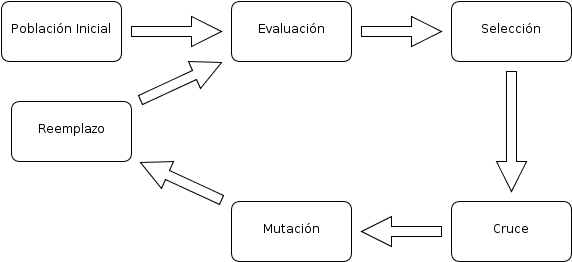
\includegraphics[scale=0.650]{./images/Dibujo1.png}
\label{modelado}
\end{center}
\end{figure}

\begin{center}
\par Figura 1: Flujo y etapas del algoritmo genético implementado.
\end{center}

\begin{figure}[H]
\begin{center}
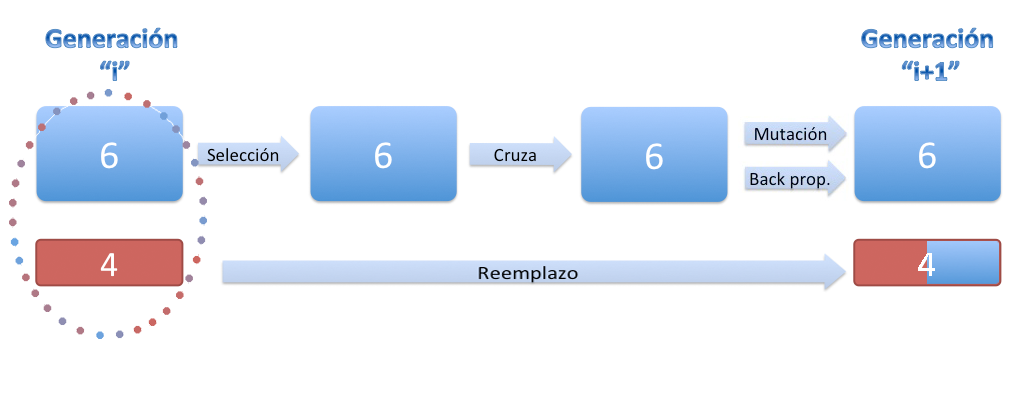
\includegraphics[scale=1.90]{./images/AlgGenModelado.png}
\label{modelado}
\end{center}
\end{figure}

\begin{center}
\par Figura 2: Modelado esquemático del funcionamiento del algoritmo genético para poblaciones de 10 individuos y un gap generacional G = 0.6.
\end{center}


\clearpage

\section*{Anexo B: Tabla de Resultados}
\begin{center} 


\begin{tabular}{| c | c | c | c | c | }
\hline
Selección & Reemplazo & Min. Entrenamiento & Min. Generalizacion & Prom. Generalización\\
\hline \hline
Ruleta & Elite & $1.6$x$10^{-3}$ & $2.5$x$10^{-3}$ & $3.0$x$10^{-3}$\\
\hline
Boltzman & Elite & $6.4$x$10^{-4}$ & $8.9$x$10^{-4}$ & $1.3$x$10^{-3}$\\
\hline
Universal & Elite & $1.7$x$10^{-3}$ & $1.9$x$10^{-3}$ & $2.1$x$10^{-3}$\\
\hline
Torneo & Elite & $7.8$x$10^{-4}$ & $9.7$x$10^{-4}$ & $1.1$x$10^{-3}$\\
\hline
Elite & Elite & $2.3$x$10^{-4}$ & $3.2$x$10^{-4}$ & $3.2$x$10^{-4}$\\
\hline
Ruleta & Mixed-Boltzman & $3.2$x$10^{-3}$ & $4.3$x$10^{-3}$ & $6.0$x$10^{-3}$\\
\hline
Boltzman & Mixed-Boltzman & $1.1$x$10^{-3}$ & $8.1$x$10^{-4}$ & $1.4$x$10^{-3}$\\
\hline
Universal & Mixed-Boltzman & $8.3$x$10^{-4}$ & $8.3$x$10^{-4}$ & $8.3$x$10^{-4}$\\
\hline
Elite & Mixed-Boltzman & $4.2$x$10^{-4}$ & $4.5$x$10^{-4}$ & $4.2$x$10^{-4}$\\
\hline
Ruleta & Boltzman & $1.7$x$10^{-3}$ & $2.4$x$10^{-3}$ & $3.7$x$10^{-3}$\\
\hline
Boltzman & Boltzman & $6.9$x$10^{-3}$ & $7.3$x$10^{-3}$ & $0.11$\\
\hline
Elite & Boltzman & $2.8$x$10^{-4}$ & $6.3$x$10^{-4}$ & $6.3$x$10^{-4}$\\
\hline
Universal & Boltzman & $1.8$x$10^{-3}$ & $2.3$x$10^{-3}$ & $2.4$x$10^{-3}$\\
\hline
Ruleta & Ruleta & $1.4$x$10^{-3}$ & $1.7$x$10^{-3}$ & $1.7$x$10^{-3}$\\
\hline
Elite & Ruleta & $8.9$x$10^{-4}$ & $9.5$x$10^{-4}$ & $9.5$x$10^{-4}$\\
\hline
Boltzman & Ruleta & $1.2$x$10^{-3}$ & $2.2$x$10^{-4}$ & $2.4$x$10^{-4}$\\
\hline
Universal & Ruleta & $5.2$x$10^{-3}$ & $4.7$x$10^{-3}$ & $5.2$x$10^{-3}$\\
\hline
\end{tabular}
\end{center}

\vspace{10px}

\begin{center} 
\par Tabla 1: Datos de ejecución para los distintos criterios de selección.\\
\vspace{5px}
\begin{itemize}
\centering
\item 30 cromosomas
\item Brecha generacional $0.5$.
\item 100 Generaciones (criterio de corte)
\item Probabilidad de mutación (clásica): $0.02$.
\item Probabilidad de cruce: $0.4$. Crossover anular.
\item Probabilidad de refinamiento: $0.05$.
\item $k_e = 6$ (para los ejemplos de \textit{Mixed}).
\end{itemize}
\end{center}

%\VerbatimInput{./code/calculoAb.m}



\end{document}